\documentclass[12pt]{article}
\usepackage{xeCJK}
\usepackage{graphicx}
\usepackage{appendix}


\renewcommand\abstractname{摘要}
\renewcommand\contentsname{目录}
\renewcommand\figurename{图}
\renewcommand\tablename{表}
\renewcommand\refname{参考文献}
\renewcommand\appendixpagename{附录}
\renewcommand\appendixtocname{附录}

\begin{document}
\title{我的第一课}
\author{陈一一}
\date{}
\maketitle

\tableofcontents

\begin{abstract}
这段内容为文章的摘要。
\end{abstract}

\newpage
\section{引言}
这是我的第一次课程,欢迎大家来前来试听。更多的信息可以从附录\ref{app:mafor}和附录\ref{app:theo}得到。

\begin{figure}[htb]
\centering
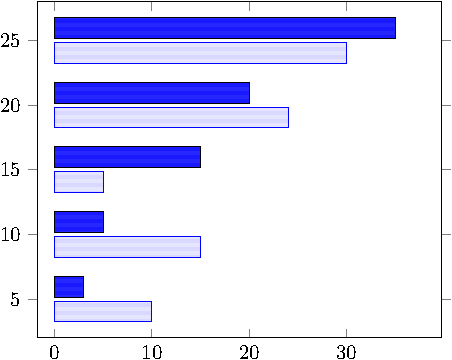
\includegraphics[scale=1]{fig1}
\caption{这是我的第一张图片}
\end{figure}

\subsection{研究背景}
表1给出了近五年水下滑翔机的市场应用占比情况\cite{Sherman2001The,Webb2001SLOCUM}。
\begin{table}[htb]
\centering
\caption{水下滑翔机应用情况}
\begin{tabular}{ccccc}
\hline
2013年&2014年&2015年&2016年&2017年\\
\hline
$15\%$&$16.5\%$&$17\%$&$18\%$&$19\%$\\
\hline
\end{tabular}
\end{table}

\subsection{研究意义}
\newpage
\bibliographystyle{unsrt}
\bibliography{cc}
\addcontentsline{toc}{section}{参考文献}

\newpage
\appendix
\appendixpage
\addappheadtotoc
\section{数学公式}\label{app:mafor}
\section{定理}\label{app:theo}

\end{document}